% This LaTeX was auto-generated from MATLAB code.
% To make changes, update the MATLAB code and export to LaTeX again.

\documentclass{article}

\usepackage[utf8]{inputenc}
\usepackage[T1]{fontenc}
\usepackage{lmodern}
\usepackage{graphicx}
\usepackage{color}
\usepackage{hyperref}
\usepackage{amsmath}
\usepackage{amsfonts}
\usepackage{epstopdf}
\usepackage[table]{xcolor}
\usepackage{matlab}

\sloppy
\epstopdfsetup{outdir=./}
\graphicspath{ {./Tutorials_3_images/} }

\matlabmultipletitles

\begin{document}

\matlabtitle{1) Plot the following 2-D sequences in MATLAB:}


\vspace{1em}
\begin{matlabcode}
clc
clear all
close all 
[n1 n2]=meshgrid(-5:5,-5:5);
\end{matlabcode}

\matlabheading{(i) Impulse.}

\begin{matlabcode}
imp=[n1==0 & n2==0]; figure; stem3(n1,n2,imp,'linewidth',2); grid; % 2D Impulse
xlabel('n_1'); ylabel('n_2'); zlabel('\delta (n_1,n_2)'); title('2D Impulse sequence');
\end{matlabcode}
\begin{center}
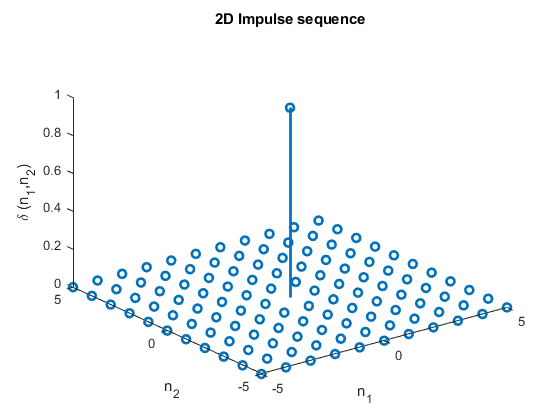
\includegraphics[width=\maxwidth{56.196688409433015em}]{figure_0.png}
\end{center}

\matlabheading{(ii) horizontal and vertical impulses.}

\begin{matlabcode}
H_imp=[n1==0]; figure; stem3(n1,n2,H_imp,'linewidth',2); grid; % 2D Horizontal Impulse 
xlabel('n_1'); ylabel('n_2'); zlabel('\delta (n_1)'); title('2D Horizontal Impulse');
\end{matlabcode}
\begin{center}
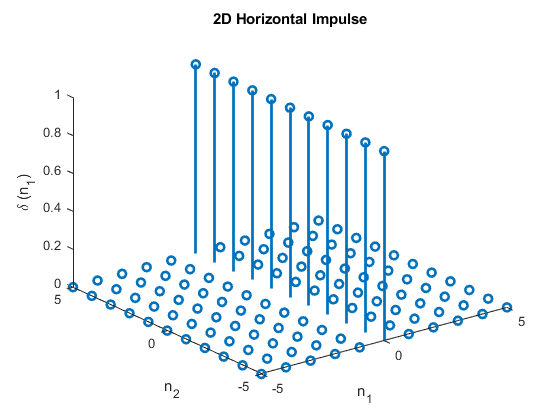
\includegraphics[width=\maxwidth{56.196688409433015em}]{figure_1.png}
\end{center}
\begin{matlabcode}
V_imp=[n2==0]; figure; stem3(n1,n2,V_imp,'linewidth',2); grid; % 2D Vertical Impulse
xlabel('n_1'); ylabel('n_2'); zlabel('\delta (n_2)'); title('2D Vertical Impulse');
\end{matlabcode}
\begin{center}
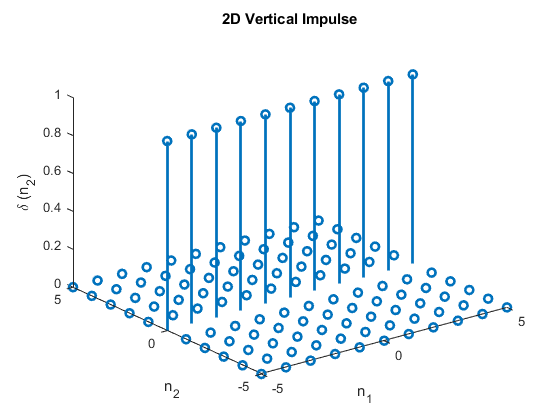
\includegraphics[width=\maxwidth{56.196688409433015em}]{figure_2.png}
\end{center}

\matlabheading{(iii) step sequence.}

\begin{matlabcode}
step=[n1>=0 & n2>=0]; figure; stem3(n1,n2,step,'linewidth',2); grid; % Step Sequence
xlabel('n_1'); ylabel('n_2'); zlabel('u(n_1,n_2)'); title('2D Unit Step sequence')
\end{matlabcode}
\begin{center}
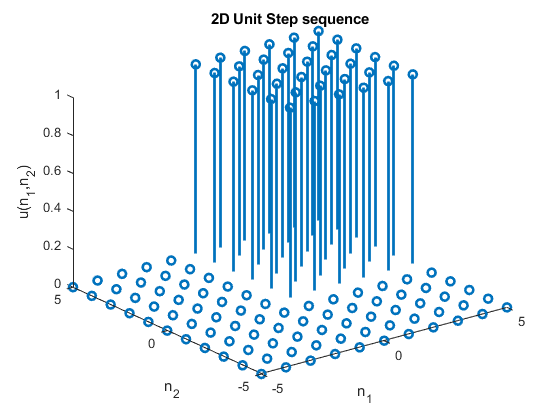
\includegraphics[width=\maxwidth{56.196688409433015em}]{figure_3.png}
\end{center}

\matlabheading{(iv) exponential sequence.}

\begin{matlabcode}
a=0.5; b=0.2;
Exp=(exp(n1)).*(exp(n2)); figure; stem3(n1,n2,Exp,'linewidth',2); grid; % 2D Exponential Seq.
xlabel('n_1'); ylabel('n_2'); zlabel('e^{(n_1,n_2)}'); title('2D Exponential sequence')
\end{matlabcode}
\begin{center}
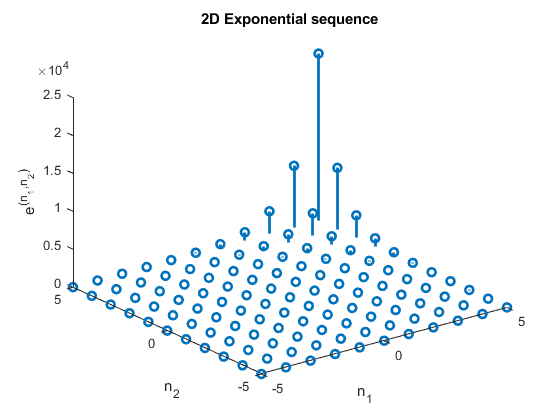
\includegraphics[width=\maxwidth{56.196688409433015em}]{figure_4.png}
\end{center}

\matlabtitle{2) Write a MATLAB code for 1-D convolution and extend this for computing 2-D convolution of separable sequences. }


\vspace{1em}
\begin{matlabcode}
xn=[7 8 9; 4 5 6; 1 2 3];
h_n1_n2=[1 -3 1; -3 9 -3; 1 -3 1];
h_n1=[1 -3 1]';
h_n2=[1 -3 1];

for i=1:3
conv_col(:,i)= Conv1D(xn(:,i)',h_n1')'; % Function code is in the last 
end

for i=1:5
conv_row(i,:) = Conv1D(conv_col(i,:),h_n2);
end
convolved2D=conv_row;
disp("Convolved 2D output using 1D convolution Row and Column wise = ");
\end{matlabcode}
\begin{matlaboutput}
Convolved 2D output using 1D convolution Row and Column wise = 
\end{matlaboutput}
\begin{matlabcode}
disp(convolved2D);
\end{matlabcode}
\begin{matlaboutput}
     7   -13    -8   -19     9
   -17    32    19    44   -21
    -4     7     5    13    -6
     1    -4     1     8    -3
     1    -1    -2    -7     3
\end{matlaboutput}
\begin{matlabcode}
out=conv2(xn,h_n1_n2,'full');
disp("Convolved 2D output directly for verification = ");
\end{matlabcode}
\begin{matlaboutput}
Convolved 2D output directly for verification = 
\end{matlaboutput}
\begin{matlabcode}
disp(out);
\end{matlabcode}
\begin{matlaboutput}
     7   -13    -8   -19     9
   -17    32    19    44   -21
    -4     7     5    13    -6
     1    -4     1     8    -3
     1    -1    -2    -7     3
\end{matlaboutput}

\begin{par}
\begin{flushleft}
3) Write a MATLAB code to separate the 2-D impulse response into 1-D impulse responses.
\end{flushleft}
\end{par}

\begin{matlabcode}
hn1n2=[1 -3 1; -3 9 -3; 1 -3 1]; %input('Enter the Matrix to be seperate into row and column vector = ')
[r c]=size(hn1n2);
if (r~=c)
    disp('Matrix must be squre matrix')
elseif (det(hn1n2)~=0)
    disp('Matrix is not singular')
else
    disp('The Matrix is seperable')
end
\end{matlabcode}
\begin{matlaboutput}
The Matrix is seperable
\end{matlaboutput}
\begin{matlabcode}
cdr=gcd(sym(hn1n2(:,1)));
cdc=gcd(sym(hn1n2(1,:)));
hn1=(1/cdr)*(hn1n2(1,:));
hn2=(1/cdc)*(hn1n2(:,1));
display(hn1, "Row Vector")
\end{matlabcode}
\begin{matlabsymbolicoutput}
Row Vector = 

\hskip1em $\displaystyle \left(\begin{array}{ccc}
1 & -3 & 1
\end{array}\right)$
\end{matlabsymbolicoutput}
\begin{matlabcode}
display(hn2, "Column Vector")
\end{matlabcode}
\begin{matlabsymbolicoutput}
Column Vector = 

\hskip1em $\displaystyle \left(\begin{array}{c}
1\\
-3\\
1
\end{array}\right)$
\end{matlabsymbolicoutput}

\matlabtitle{4) Consider a digital image of size 512 × 512 and apply the amplitude quantization at }


\vspace{1em}
\matlabheading{(i) 8 bits/pixel, }

\begin{matlabcode}
[I1 map]=imread("lenna.bmp");
figure; imshow(I1,map); title("Original image");
\end{matlabcode}
\begin{center}
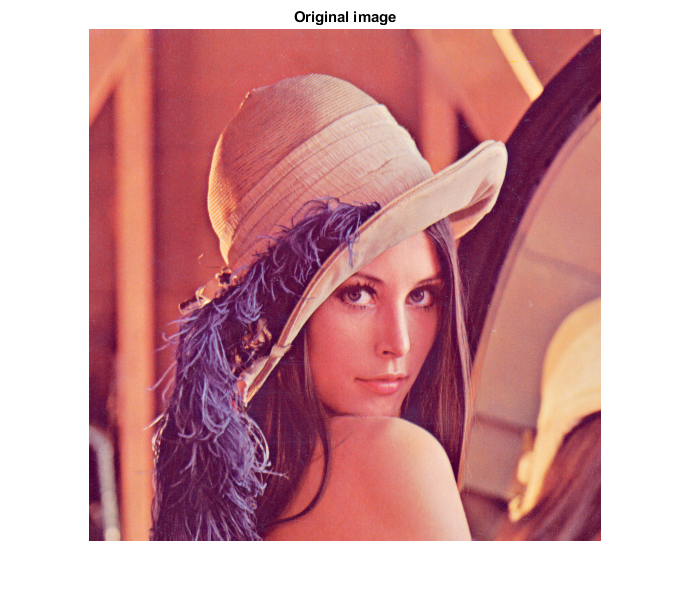
\includegraphics[width=\maxwidth{69.44305067737079em}]{figure_5.png}
\end{center}
\begin{matlabcode}
[r c ch] = size(I1);
if ch>=2;
    I1=rgb2gray(I1);
%     figure; imshow(I1); title("GreyScal image");
end

thresh=multithresh(I1,8); % Calculating Thresholds for 8 bits
seg_I=imquantize(I1,thresh); % Applying thresholds to obtain segmented image
RGB=label2rgb(seg_I); % Assigning the RGB color to the labels
figure; subplot(221); imshow(RGB); title("Segmented image 8bits/[pixel");
\end{matlabcode}

\begin{par}
\begin{flushleft}
(ii) 6 bits/pixel.
\end{flushleft}
\end{par}

\begin{matlabcode}
thresh=multithresh(I1,6); % Calculating Thresholds for 6 bits
seg_I=imquantize(I1,thresh); % Applying the thresholds to obtain segmented image
RGB=label2rgb(seg_I); % Assigning the RGB color to the labels
subplot(222); imshow(RGB); title("Segmented image 6bits/[pixel");
\end{matlabcode}

\begin{par}
\begin{flushleft}
(iii) 2 bits/ pixel.
\end{flushleft}
\end{par}

\begin{matlabcode}
thresh=multithresh(I1,2); % Calculating Thresholds for 2 bits
seg_I=imquantize(I1,thresh); % Applying the thresholds to obtain segmented image
RGB=label2rgb(seg_I); % Assigning the RGB color to the labels
subplot(223); imshow(RGB); title("Segmented image 2bits/[pixel");
\end{matlabcode}

\begin{par}
\begin{flushleft}
(iv) 1 bit/pixel. 
\end{flushleft}
\end{par}

\begin{matlabcode}
thresh=multithresh(I1,1); % Calculating Thresholds for 1 bits
seg_I=imquantize(I1,thresh); % Apply the thresholds to obtain segmented image
RGB=label2rgb(seg_I); % Assigning the RGB color to the labels
subplot(224); imshow(RGB); title("Segmented image 1bit/[pixel");
\end{matlabcode}
\begin{center}
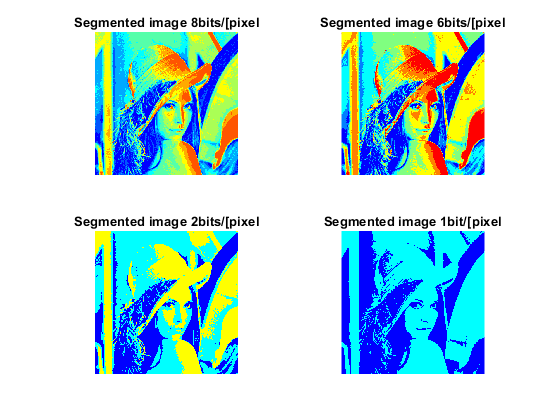
\includegraphics[width=\maxwidth{56.196688409433015em}]{figure_6.png}
\end{center}

\matlabheading{Conclusion : Thare is a significant change in the color / intevsity image for diffrent number of bits/pixels}


\vspace{1em}
\matlabtitle{5) Consider a digital image of size 512 X 512 and reduce pixels to (i) 256 X 256, (ii) 128 X 128, (iii)}

\matlabtitle{64 X 64, (iv) 32 X 32. Comment on the variation on the image.}


\vspace{1em}
\begin{matlabcode}
I=imread("peppers.png"); % Reading Image of size 512x512
figure; imshow(I); title("Original image 512 x 512");
\end{matlabcode}
\begin{center}
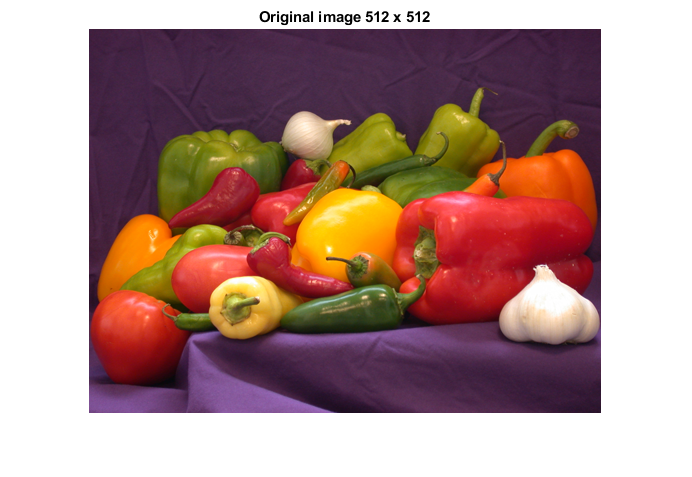
\includegraphics[width=\maxwidth{69.44305067737079em}]{figure_7.png}
\end{center}
\begin{matlabcode}

I_256=imresize(I,0.5); % Resizing Image for size 256x256.
figure; imshow(I_256); title("Resized image 256 x 256");
\end{matlabcode}
\begin{center}
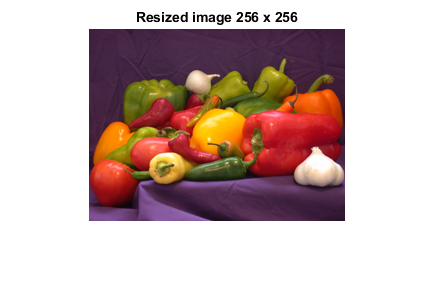
\includegraphics[width=\maxwidth{43.753135975915704em}]{figure_8.png}
\end{center}
\begin{matlabcode}

I_128=imresize(I,0.25); % Resizing Image for size 128x128
figure; imshow(I_128); title("Resized image 128 x 128");
\end{matlabcode}
\begin{center}
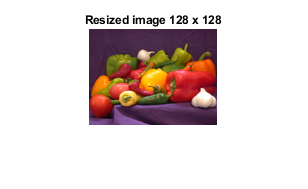
\includegraphics[width=\maxwidth{30.90817862518816em}]{figure_9.png}
\end{center}
\begin{matlabcode}

I_64=imresize(I,0.125); % Resizing Image for size 64x64
figure; imshow(I_64); title("Resized image 64 x 64");
\end{matlabcode}
\begin{center}
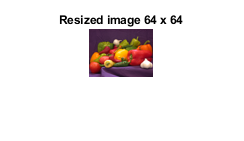
\includegraphics[width=\maxwidth{24.485699949824387em}]{figure_10.png}
\end{center}
\begin{matlabcode}

I_32=imresize(I,0.0625); % Resizing Image for size 32x32
figure; imshow(I_32); title("Resized image 32 x 32");
\end{matlabcode}
\begin{center}
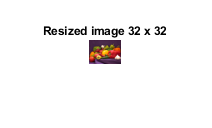
\includegraphics[width=\maxwidth{21.274460612142498em}]{figure_11.png}
\end{center}

\matlabtitle{6) Use an image file of your choice and pass it through a low-pass filter whose impulse response is}

\matlabtitle{given in Fig. 1, and observe the output.}

\matlabtitle{                                                       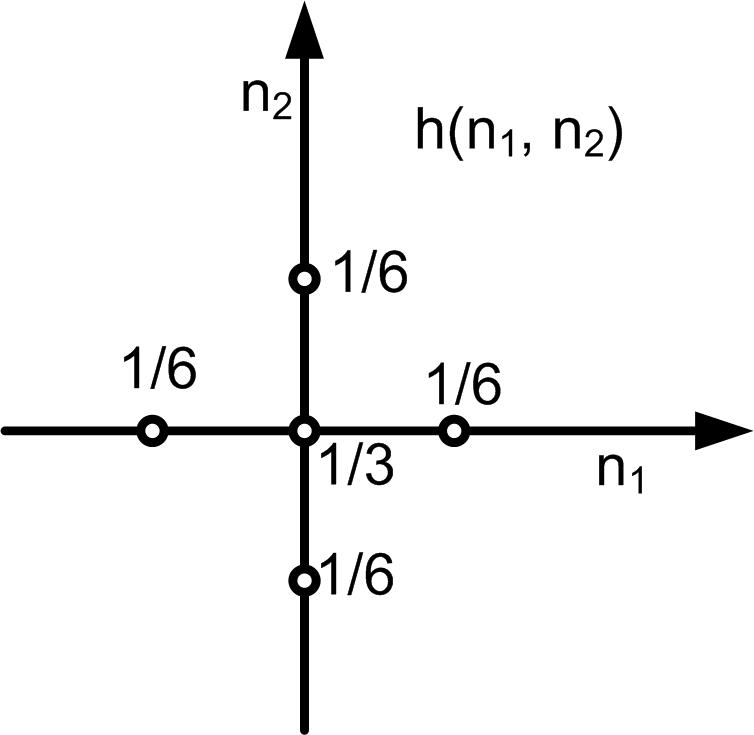
\includegraphics[width=\maxwidth{29.001505268439537em}]{image_0}}

\begin{par}
\begin{flushleft}
                                                                                                      Fig. 1. Low-pass filter impulse response
\end{flushleft}
\end{par}


\vspace{1em}
\begin{matlabcode}
I_512 =  imread('peppers.png'); % Reading Image in RGB format  
LPF = [0 1/6 0;1/6 1/3 1/6;0 1/6 0]; % Creating LFP
Io = imfilter(I_512,LPF); % Passing image throgh LPF.

Ig = rgb2gray(I_512); % Converting from RGB to Gray scale image.
Iout = uint8(round(conv2(Ig, LPF, 'same')));  % Filtering Image throgh LPF
figure; imshow(I_512); title('Original Image'); % Plotting Origibal Image
\end{matlabcode}
\begin{center}
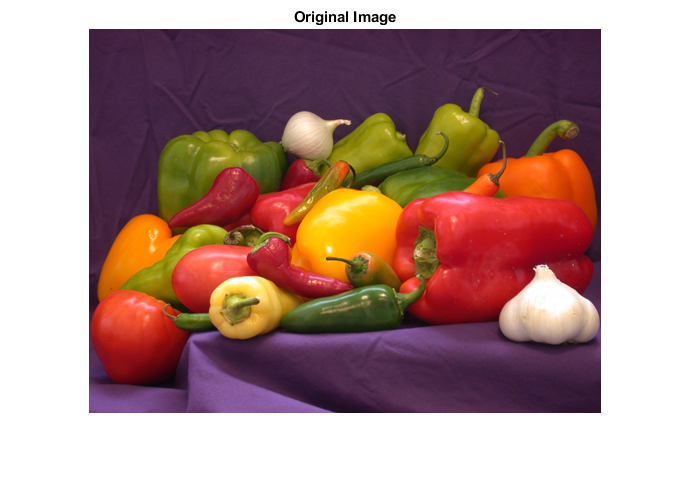
\includegraphics[width=\maxwidth{69.44305067737079em}]{figure_12.png}
\end{center}
\begin{matlabcode}
figure; imshow(Io); title('LPF Image, using inbuilt command'); % LPF'ed Image
\end{matlabcode}
\begin{center}
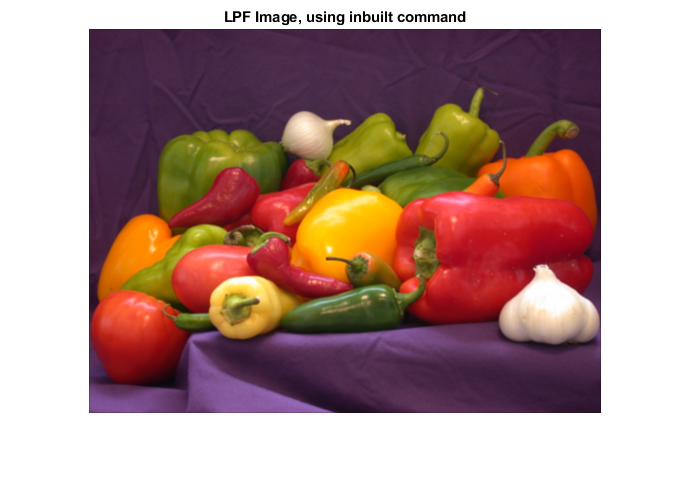
\includegraphics[width=\maxwidth{69.44305067737079em}]{figure_13.png}
\end{center}

\matlabheading{Conclusion : Filtered Image throgh LFP, got Blurred compare to Original Image}


\vspace{1em}
\begin{matlabcode}
figure; imshow(Ig); title('Grayscal Image'); % Plotting Grayscal Image
\end{matlabcode}
\begin{center}
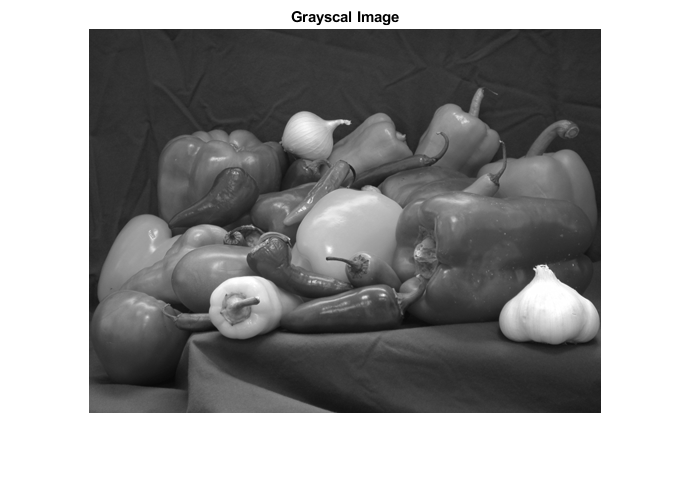
\includegraphics[width=\maxwidth{69.44305067737079em}]{figure_14.png}
\end{center}
\begin{matlabcode}
figure; imshow(Iout); title('LPF Image, using convolution Method'); % LPF Image using Convolution method
\end{matlabcode}
\begin{center}
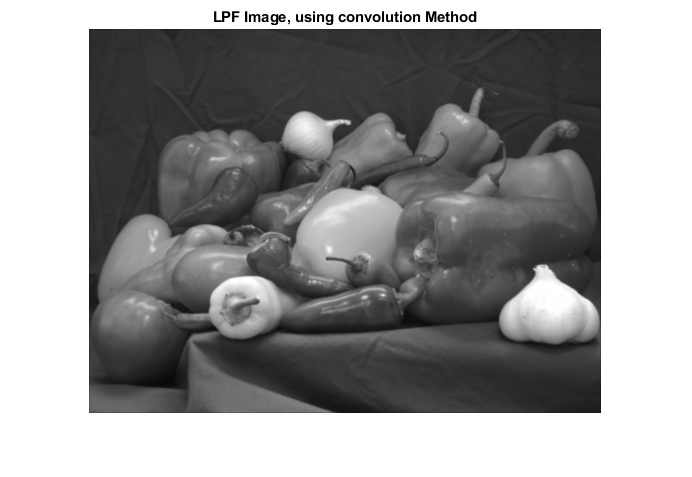
\includegraphics[width=\maxwidth{69.44305067737079em}]{figure_15.png}
\end{center}

\matlabheading{Conclusion : Filtered Image throgh LFP, got Blurred compare to Original Image}


\vspace{1em}
\matlabtitle{7) Use an image file of your choice and pass it through a high-pass filter whose impulse response is}

\matlabtitle{given in Fig. 2, and comment on the output.}

\begin{par}
\begin{flushleft}
                                                                                                                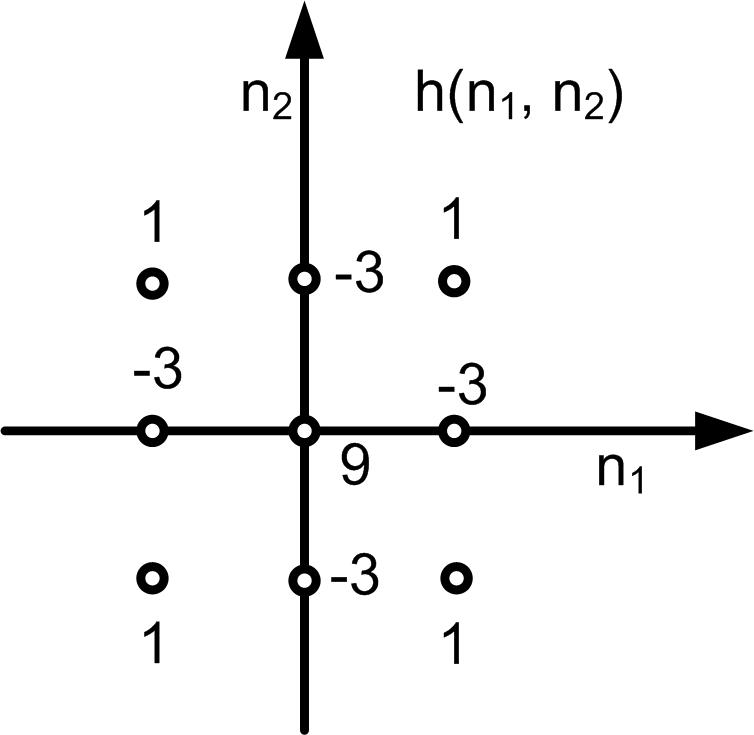
\includegraphics[width=\maxwidth{27.094831911690918em}]{image_1}
\end{flushleft}
\end{par}

\begin{par}
\begin{flushleft}
                                                                                                                   Fig. 2. High-pass filter impulse response
\end{flushleft}
\end{par}

\begin{matlabcode}
Ig =  imread('riceblurred.png'); % Reading Image in RGB format  
figure; imshow(Ig); title('Original Image'); % Plotting Origibal Image
\end{matlabcode}
\begin{center}
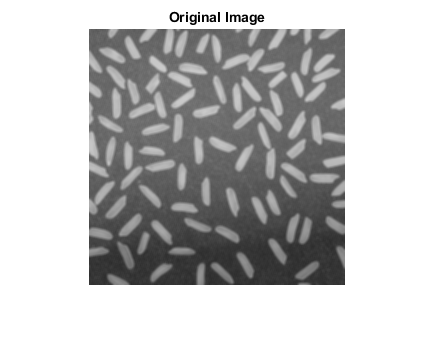
\includegraphics[width=\maxwidth{43.753135975915704em}]{figure_16.png}
\end{center}
\begin{matlabcode}
HPF=[1 -3 1;-3 9 -3;1 -3 1]; % Creating HPF
Io = imfilter(Ig,HPF); % Passing Image Throgh HPF
figure; imshow(Io); title('HPF Image, using inbuilt command') % HPF Image, using inbuilt command
\end{matlabcode}
\begin{center}
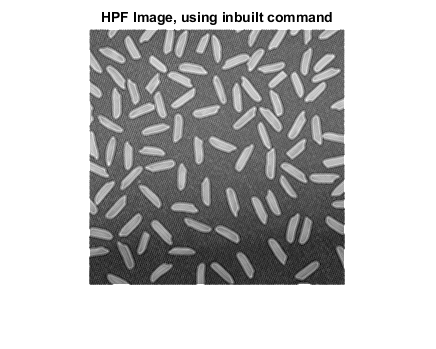
\includegraphics[width=\maxwidth{43.753135975915704em}]{figure_17.png}
\end{center}
\begin{matlabcode}
Iout = uint8(round(conv2(Ig, HPF, 'same'))); % Convolving Image with HPF
figure; imshow(Iout); title('HPF Image, using convolution Method') % HPF Image, using convolution Method
\end{matlabcode}
\begin{center}
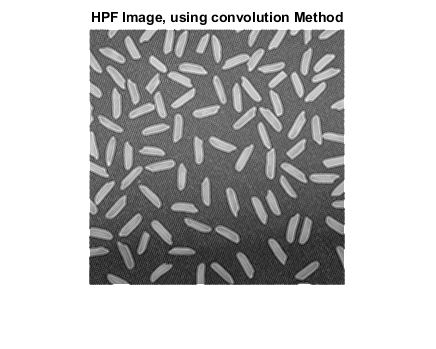
\includegraphics[width=\maxwidth{43.753135975915704em}]{figure_18.png}
\end{center}

\matlabheading{Conclusion : Image got Sharpen after Paassing throgh HPF}

\vspace{1em}


\vspace{1em}

\matlabtitle{Function for 1D Convolution }

\begin{matlabcode}
function yn = Conv1D(xn,hn)
m=length(xn);
n=length(hn);
X=[xn,zeros(1,n)];
H=[hn,zeros(1,m)]; 
for i=1:n+m-1
    yn(i)=0;
    for j=1:m;
        if(i-j+1>0)
            yn(i)=yn(i)+X(j)*H(i-j+1);
        else
        end
    end
end
end
\end{matlabcode}

\end{document}
